\begin{questions}

\question Consider the first-order linear differential equation
$$y' -\dfrac{3}{x}y = x^4.$$
\begin{parts}
\part[8] Find the general solution of the differential equation.
\vfill
\vfill
\part[3] Find the particular solution that satisfies the initial condition $y(1) = 5.$
\vfill
\end{parts}

\newpage

\question[8] For your retirement ``nest egg,'' you deposit \$300 at the end of each month into a
bank account paying 6\% interest compounded monthly. Use your knowledge of series to find an

expression that represents the amount of this annuity at the end of your 40-year working career.
While you do not need to simplify your final answer, you do need to find a single term
expression that represents the value of the annuity. Writing your answer as a sum of terms is
not enough.
%sec 10.2
\newpage
\question
\begin{parts}
\part[6] Find the 3rd degree Taylor polynomial of $f(x) = \sqrt{x}$ centered at $x=9.$
\vfill
\part[4] Use the 3rd degree Taylor polynomial that you found in part (a) to find an approximation
for $\sqrt{10}$ by evaluating the polynomial at an appropriate value of $x.$
\vfill
\end{parts}
\newpage
\question[7] Use known series expansions to find the Taylor Series of $f(x) = x^2 e^{2x}$
centered at $x=0.$ Give at least the first five terms of the series.
\newpage
\question[8] Find the volume under the surface $f(x,y) = 4y$ and above the shaded region $R$
shown in the graph.
%Note to Kailtyn: can you help me with a picture of the region between xsquared and sqrtx?
%-Done.

\begin{tikzpicture}
\begin{axis}[
axis lines = middle,


xmin=0, xmax=2,


ymin=0, ymax=2,


xtick distance=1, ytick distance=1, grid=both ]

\addplot [domain=0:1.3, samples=100,->, name path=f, thick]
{sqrt(x)} node[pos=1, right]{$y=\sqrt{x}$};;
\addplot [domain=0:1.3, samples=100,->, name path=g, thick]
{x^2} node[pos=1, above]{$y=x^2$};
%\node[font=\footnotesize] at (axis cs: 2,1.5) {$y=f(x)$};
%\node[ font=\footnotesize] at (axis cs: 1.5,2.2) {$y=g(x)$};
\addplot[gray!50, opacity=0.4] fill between[of=f and g, soft clip={domain=-1:1}];
\node at (axis cs:0.5, 0.5) {$R$};

\end{axis}
\end{tikzpicture}

\newpage

\question[10] Use the method of Lagrange multipliers to find the minimum of $f(x,y) = 4xy$
subject to the constraint $2x+6y=12.$
\newpage
\question[8] Consider the initial-value problem
$$y' = 2x + y, \,\, y(0) = 2.$$
Use Euler’s method with $n = 2$ steps to approximate $y(1).$
\newpage
\question[8] Consider the function $f(x) = x^2-x-2.$
Use 2 iterations of Newton’s method starting with $x_0 = 1$ to approximate a zero of $f(x).$
\newpage
\question Consider a continuous random variable $X$ with probability density function $f(x) =
\dfrac{3}{2}\sqrt{x}$ on $[0,1].$
\begin{parts}
\part[5] Compute the probability $P\left(X \ge \dfrac{1}{2} \right)$

\vfill
\part[5] Find the mean (i.e., the expected value) of $X.$
\vfill
\end{parts}

\newpage

\question For the spinner below, the arrow is spun and then stops, pointing in one of the
numbered sectors, with probability proportional to the area of the sector. Let $X$ stand for the
number so chosen. Find the following. (Leave your answers as fractions, integers, or exact
decimals.)
\vspace{0.5in}
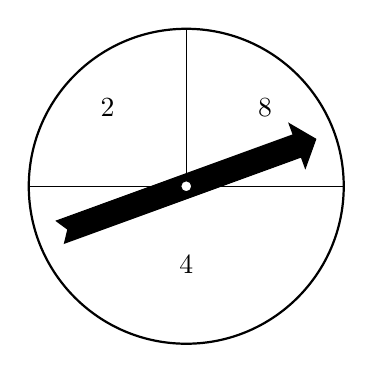
\begin{tikzpicture}
\draw[fill=none,thick](0,0) circle (2.0);
\draw[](-2,0) -- (2,0);
\draw[] (0,0) --(0,2);
%\draw[-{Triangle[width=16pt,length=10pt]}, line width=8pt](-1.5, -0.5) -- (1.5, 0.5);
\draw[fill=black, rotate=20]
(-1.7,0.15)--(-1.6,0)--(-1.7,-0.15)--(1.5,-0.15)--(1.5,-0.3)--(1.75,0)--(1.5,0.3)--(1.5,0.15)--cycle;
\draw[fill=white](0,0) circle (2 pt);
\node at (1,1) {8};
\node at (-1,1) {2};
\node at (0,-1) {4};
\end{tikzpicture}
\vspace{0.5in}
\begin{parts}
\part[2] $P(X=8)=$
\vfill
\part[4] $E(X)=$
\vfill

\end{parts}
%Consider the experiment of rolling two fair 6-sided dice.
%\begin{parts}
%\part[3] Determine the probability that the sum of the numbers rolled is 10.
%\vfill
%\part[3] Determine the probability that a 1 is rolled on either die.
%\vfill
%\end{parts}

\newpage

\question A company's profit $P(x,y)$ from making $x$ computers and $y$ tablets per day is
given by $P(x,y) = 4x^2-5xy +5y^2 +10x+4y+70.$
\begin{parts}
\part[3] Find the marginal profit function for computers.
\vfill
\part[3] Find the marginal profit function for tablets.
\vfill
\end{parts}
\newpage

\question Clearly mark the correct answer for each of the following by completely filling in the
appropriate bubble. \textbf{No justification is needed.}
\bigskip
\begin{parts}

\part[2] Consider the infinite series $\displaystyle\sum_{n=0}^{\infty}\dfrac{8}{6^n}.$ What can
you say about the convergence of this series?

\begin{itemize}[label={}]
\item \chooseone The series converges to $8/6.$
\item \chooseone The series converges to $\frac{8}{1-1/6}.$
\item \chooseone The series converges, but its value cannot be determined.
\item \chooseone The series diverges.
%\item \chooseone It cannot be determined whether the series converges or diverges with the
%given information.
\end{itemize}
\vfill
\part[2] Consider the infinite series $\displaystyle\sum_{n=1}^{\infty}(-1)^{n-1}\dfrac{1}{n2^n}.$
What can you say about the convergence of this series?
\begin{itemize}[label={}]
\item \chooseone The series converges to $\ln(3/2).$
\item \chooseone The series converges to $\frac{1}{1-1/2}.$
\item \chooseone The series converges, but its value cannot be determined.
\item \chooseone The series diverges.
%\item \chooseone It cannot be determined whether the series converges or diverges with the
%given information.
\end{itemize}
\vfill

\part[2] The value of a painting, initially worth \$10000, continuously grows in value at a rate of
4\% a year. Let $y(t)$ be the value of the painting after $t$ years. Which of the following
expressions correctly describe $y(t)$? Select all that apply.
\begin{itemize}[label={}]
\item \choosemany $y(t)= 10000e^{0.04t}$
\item \choosemany $y(t)= 10000(1+0.04/n)^{nt}$
\item \choosemany $y'(t) = 0.04(10000 -y).$
\item \choosemany $y'(t) = 0.04y,$ with $y(0) = 10000$
\item \choosemany None of the above.

\end{itemize}
\vfill

\part[2] Consider the function $f(x,y) = e^{x-1}\sqrt{y -4}.$ Then the domain of $f(x,y)$ is given
by:

\begin{itemize}[label={}]
\item \chooseone $\{ (x,y) | y \neq 4 \}$
\item \chooseone $\{ (x,y) | x \neq 1\, \text{and } \, y \neq 4 \}$
\item \chooseone $\{ (x,y) | y > 4 \}$
\item \chooseone $\{ (x,y) | y \ge 4 \}$
\item \chooseone $\{ (x,y) | y \le 4 \}$
\item \chooseone $\{ (x,y) | x \ge 1 \}$
\item \chooseone $\{ (x,y) | x \le 1 \}$
\item \chooseone None of the above.

\end{itemize}
\vfill

\end{parts}

\newpage
\end{questions}
